\chapter{Blanket blocking}
Il \emph{blanket blocking} � un attacco che permette di bloccare l'accesso all'intera rete Tor e viene solitamente attuato da enti governativi, ISP o amministratori di rete. Esso non intende colpire un router o un client specifico, ma attraverso l'utilizzo di firewall o filtri impedisce l'accesso a chiunque si voglia collegare alla rete Tor.
%Esistono vari metodi che impediscono l'accesso alla rete:
%\begin{itemize}
%\item bloccando le connessioni verso le directory authorities;
%\item bloccando le connessioni verso i router distribuiti dalle directory authorities;
%\item filtrando i pacchetti che nell'header HTTP contengono dei riferimenti a Tor;
%\item bloccando l'accesso al sito ufficiale di Tor, per diminuire il numero di download del software;
%\item \textcolor{green}{tecniche DPI}
%\end{itemize}
Esistono principalmente due metodi per impedirne l'accesso:
\begin{itemize}
\item blocco delle connessioni verso le infrastrutture di Tor (\emph{address-blocking});
\item utilizzo di tecniche DPI (\emph{content-based blocking}).
\end{itemize}
Per attuare il primo metodo, un ISP (ad esempio) pu� semplicemente inserire in una blacklist tutte le coppie IP:porta delle directory authorities, gli IP distribuiti da esse o l'IP del server che ospita il sito \url{https://www.torproject.org/} (per impedire che il software si diffonda). Ogni qualvolta si tenter� di stabilire una connessione verso uno di questi indirizzi IP, verr� impedito ai pacchetti di raggiungere il server, oppure di ricevere le risposte. Con le tecniche DPI (Deep Packet Inspection) i pacchetti vengono analizzati da software specifici in grado di individuare il contenuto del pacchetto o l'applicazione che l'ha generato (in questo caso Tor) e scartarli per impedire che arrivino a destinazione. Nel caso di Tor, solitamente, viene individuato il protocollo nel momento in cui il client invia la cipher list al primo router, contenuta nel TLS hello\footnote{Il TLS hello � la prima fase dell'handshake TLS, in cui il client comunica al server (o al router in questo caso) gli algoritmi crittografici supportati, la versione TLS ecc.}. Infatti la cipher list sembra essere unica ed utilizzata solamente da Tor.

\section{Bridge}
Il metodo pi� semplice per difendersi da questo tipo di attacco consiste nell'utilizzare i bridge. Essi sono dei router Tor, che non vengono inseriti nelle liste delle directory authorities. Dato che i loro indirizzi IP non sono pubblici, non vengono censurati e quindi � possibile utilizzarli come first-hop per collegarsi alla rete Tor. Per ovvi motivi vengono messi a disposizione dei metodi che permettono di ottenere solamente pochi bridge alla volta. Inviando un' email a \mail{bridges@torproject.org} da un account Riseup, Gmail o Yahoo si ottiene una risposta con tre indirizzi IP di tre bridge diversi. Oppure vengono distribuiti attraverso server HTTPS come \url{https://bridges.torproject.org/}, social networks o canali privati. 

Un metodo molto pi� sofisticato \cite{torbridge} per raccogliere gli indirizzi IP dei bridge, � quello di utilizzare un middle router controllato che raccolga informazioni sugli altri router della rete: inserendo all'interno della rete un router con un bitrate elevato si avr� un alta probabilit� che esso venga scelto come middle nelle costruzioni dei path. Cos� facendo il router controllato pu� confrontare gli indirizzi IP dei nodi di ingresso con quelli delle directory authorities. Se l'indirizzo confrontato non � presente tra quelli pubblici allora il router d'ingresso � un bridge e quindi pu� essere comunicato attraverso un'email ad un indirizzo prestabilito. Quando gli onion router notano che il bitrate e l'uptime del router controllato stanno al di sopra di un valore medio, esso viene etichettato come entry router dai directory server. Per evitare che il nodo inserito all'interno della rete diventi un entry bisogna regolare il bitrate e l'uptime dinamicamente, mentre per evitare che diventi un exit � necessario indicarlo in fase di configurazione.
% FIGURA
\begin{figure}[!htbp]
\centering
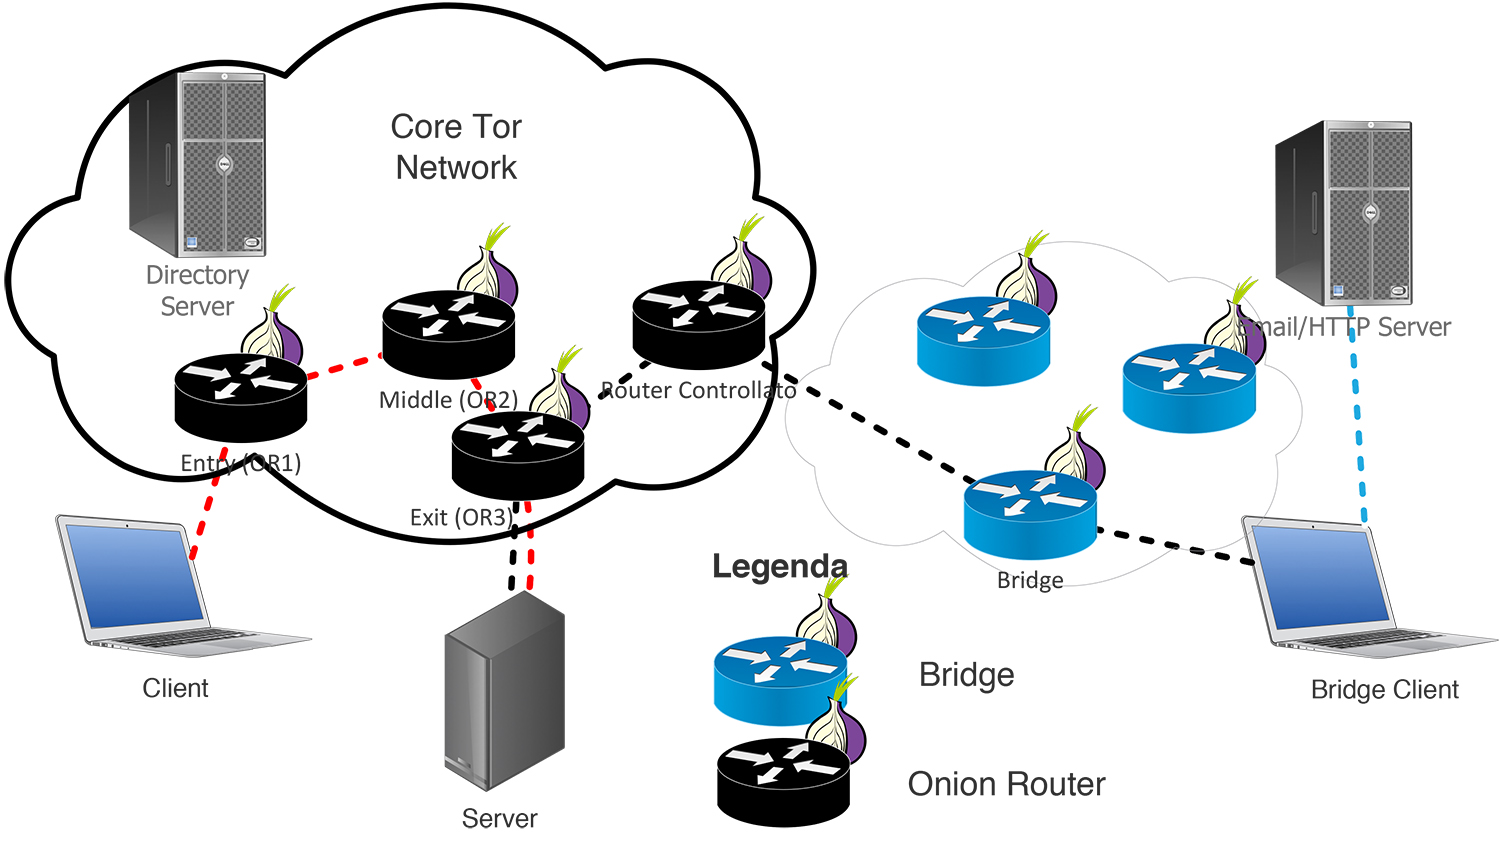
\includegraphics[width=0.6\textwidth]{./figure//middleroutercut2}
\caption{Scenario di rete con router controllato.}
\label{FIG:TorBridge}
\end{figure}
\\Analizziamo allora la \textbf{probabilit� di cattura}, ovvero la probabilit� che un circuito che sceglie come first-hop un bridge, attraversi il router controllato. Ipotizziamo di inserire $k$ middle router nella rete e che il numero totale di OR fino a quel momento fosse $N$, allora i rispettivi bitrate li indicheremo con $\{B\ped{1},B\ped{2}, ... , B_{k}, B_{k+1}, ... , B_{k+N}\}$. Tutti i router inseriti avranno lo stesso bitrate, $B_1 = B_2 = ... = B_k = b$. Definiamo $B$ come la somma dei bitrate di tutti gli OR originariamente presenti nella rete: $B = \sum_{i=k+1}^{k+N} B_i$. Quindi dopo l'inserimento, il bitrate totale sar� $B+k \cdot b$. Da \eqref{eqn:wepath} e \eqref{eqn:wgpath} possiamo scrivere:

\begin{equation}
W_E=
\begin{cases}
1-\frac{B+k \cdot b}{3 \cdot (B_{E0}+B_A)},      	& \text{se $W_E>0$,} \\
0, 									& \text{se $W_E\le0$.}
\end{cases}
\end{equation}

\begin{equation}
W_G=
\begin{cases}
1-\frac{B+k \cdot b}{3 \cdot (B_{G0}+B_A)},      	& \text{se $W_G>0$,} \\
0, 									& \text{se $W_G\le0$.}
\end{cases}
\end{equation}
Diamo allora la definizione di probabilit� di cattura:

\begin{teorema}[Probabilit� di cattura]
\begin{equation}
\label{eqn:probcatch}
P(k,b) = \frac{k\cdot b}{B_{E0} \cdot W_E + B_A \cdot W_E \cdot W_G + B_{G0} \cdot W_G + (B_N+ k \cdot B)}
\end{equation}
\end{teorema}
Da qui deriva immediatamente che pi� � grande il bitrate portato all'interno della rete, pi� probabilit� si ha di essere scelti nei circuiti Tor, come enunciato dal seguente teorema.

\begin{teorema}
La probabilit� di cattura � determinata dall'ammontare del bitrate aggiunto dagli $OR$ controllati. Sia $M = k \cdot b, M' = k' \cdot b' \ con \ M \ge M'$,
\begin{equation}
\label{eqn:ammband}
P(M) \ge P(M').
\end{equation}
L'uguaglianza si ha con $M'=M$.
\end{teorema}

\begin{teorema}
Dopo la creazione di q circuiti, la probabilit� che almeno uno dei bridge si sia collegato ad uno dei router controllati �:
\begin{equation}
\label{eqn:ammband}
P(k,b,q) = 1- (1-P(k,b))^{q}, \ q=1,2,3,...
\end{equation}
\end{teorema}
In conclusione, la probabilit� di cattura aumenta con l'aumentare del bitrate totale dei router controllati e con il numero di circuiti che vengono creati.
Come � stato evidenziato sperimentalmente \cite{torbridge}, in pochi giorni con un solo router si � in grado di raccogliere un numero considerevole di bridge.

\section{Pluggable transports}
Il semplice uso dei bridge si oppone solo alla censura a livello IP e non va a contrastare, laddove vengono utilizzate, le tecniche DPI. Come abbiamo detto il Deep Packet Inspection va ad analizzare il contenuto dei pacchetti, ma � possibile camuffarli con dei tool detti \emph{pluggable transports}  in modo da aggirare i blocchi di tipo content-based.
Possono essere scelte due strategie per camuffare i pacchetti:
\begin{itemize}
\item far sembrare il flusso di pacchetti qualcosa che non viene bloccato;
\item far sembrare il flusso di pacchetti qualcosa di autorizzato.
\end{itemize}
Dei tool che realizzano la prima strategia sono: obfs2, obfs3, ScrambleSuit e obfs4 che cercano di camuffare i pacchetti facendo sembrare lo stream di byte un insieme uniforme di bit casuali, inoltre fanno in modo che non rimanga nessuna parte della comunicazione in chiaro, neanche nella fase di handshake TLS e nello scambio delle chiavi. Anche se � possibile decifrare lo stream, questo richiederebbe ulteriori risorse che non vengono impiegate nella maggior parte dei casi. Questo metodo richiede che il tool sia eseguito sia sul client che sul bridge a cui ci si vuole collegare.
Nel secondo caso vengono usate tecniche steganografiche, che "trasformano" lo stream di dati di Tor, in uno stream simile a quello di altre applicazioni com ad esempio Skype.  

\section{Great Firewall of China (GFC)}
\emph{Great Firewall of China} � un termine utilizzato per far riferimento al \emph{Golden Shield Project}, un progetto per il controllo e la censura di Internet sviluppato dal governo cinese. Esso merita un approfondimento a parte per quanto riguarda l'aspetto tecnico data la sua efficacia nel realizzare il blanket blocking. Ogni volta che un client all'interno del territorio cinese tenta di collegarsi ad un $OR$, un blocco DPI identifica il protocollo Tor durante lo scambio della cipher suite TLS e lo comunica a dei server. Questi server provano a collegarsi all'$OR$ con lo stesso protocollo e, se ci riescono, lo inseriscono in una blacklist. Questo vale anche quando qualcuno ci si collega ad un bridge, rendendoli quindi inutilizzabili. I directory authorities vengono bloccati a livello IP, infatti non rispondono n� a pacchetti TCP n� ICMP. Attualmente il GFC sembra lasciar passare il TCP SYN, ma eliminare il SYN/ACK inviato dal router al client e la stessa cosa sembra succedere quando si prova a collegarsi ad un bridge bloccato. Comunque il blocco di router e bridge sembra riferirsi alle tuple IP:porta, dato che essi rispondono al ping verso altre porte. Probabilmente questa scelta � stata fatta per minimizzare gli effetti collaterali dovuti alla censura.

\subsection{Contromisure}
I risultati sperimentali \cite{gfc} mostrano che una tupla IP:Porta rimane bloccata fintanto che � raggiungibile. Questo significa che periodicamente i server del GFC provano a stabilire delle connessioni con i router/bridge che avevano precedentemente inserito nella blacklist. Se vedono che non sono pi� raggiungibili rimuovono il blocco. Questo meccanismo pu� essere sfruttato per aggirare il firewall. Si pu� pensare di inserire un router all'interno della rete Tor posizionato al di fuori del territorio cinese e configurarlo in modo che accetti solo connessioni da degli indirizzi IP prestabiliti. Cos� facendo anche se i blocchi DPI rilevassero l'uso del protocollo Tor verso il router, i server del GFC non potrebbero provare a collegarsi dato che le loro richieste verrebbero scartate e quindi non bloccherebbero il router.

Il progetto Tor ha anche sviluppato un tool chiamato \emph{meek} \cite{meek, domainfronting} in grado di codificare uno stream di dati come una sequenza HTTPS di richieste e risposte che vengono inoltrate da un web server; questa tecnica � detta \emph{domain fronting}.
% FIGURA
\begin{figure}[!htbp]
\centering
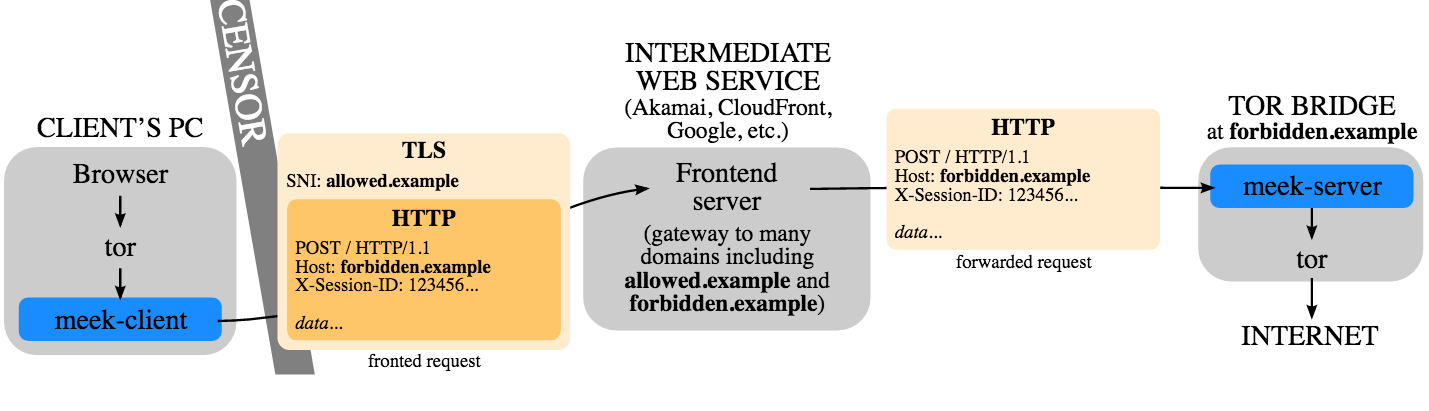
\includegraphics[width=0.9\textwidth]{./figure//meek-diagram}
\caption{Schema di funzionamento del tool meek.}
\label{FIG:meek}
\end{figure}
Il server quindi ha la funzione di intermediario e permette ad un client di collegarsi ad un Tor bridge, facendo sembrare che le richieste vadano verso un IP autorizzato. Meek si compone di due parti: meek-client e meek-server. La parte client � un processo separato rispetto al browser Tor che riceve i dati da trasmettere da esso, li "impacchetta" dentro ad una richiesta POST e li invia al bridge attraverso il web server. Il dominio autorizzato viene messo "all'esterno" della richiesta: nella query DNS e nell'estensione SNI TLS \footnote{L'estensione SNI (Server Name Indication) � un'estensione del protocollo TLS con cui un client indica a quale hostname sta cercando di connettersi all'inizio della fase di handshake.}, mentre il dominio vietato "all'interno": nell' host header della richiesta HTTP. Sul bridge � in esecuzione la parte server di meek, che decodifica le richieste HTTP in ingresso e le invia nella rete Tor. Dopo aver ricevuto una richiesta, meek-server controlla se il bridge ha dei dati da inviare come risposta al client, e li invia nella risposta HTTP; quando meek-client riceve la risposta, ne passa il corpo al processo Tor. Il motivo per cui questi web server non vengono bloccati � che fanno parte di qualche CDN, chi censura quindi, incapace di distinguere tra traffico fronted e non fronted, � costretto a scegliere: permettere il passaggio di traffico che aggira i firewall o bloccare completamente interi domini, con pesanti effetti collaterali. 


% ----------------------  ESEMPI UTILI PRONTI ALL'USO  ----------------------
%QUARTO capitolo della tesi. Esempio di citazione doppia \cite{Munoz-Lipo,Vas}.
%
%Esempio di figura in \figurename\ \ref{FIG:LogoUniPD}.
%
%\begin{figure}[!htbp]
%\centering
%
\includegraphics[width=0.25\textwidth]{./figure//LogoUniPD}
%\caption{Esempio di figura.}
%\label{FIG:LogoUniPD}
%\end{figure}
%
%Esempio di tabella in \tablename\ \ref{TAB:Esempio}.
%
%\begin{table}[!htbp]
%\centering
%\renewcommand{\arraystretch}{1.3}
%\caption{Esempio di tabella.}
%\begin{tabular}{cc}
%\hline
%Nome & Valore \\
%\hline
%a & 1 \\
%b & 2 \\
%c & 3 \\
%d & 4 \\
%e & 5 \\
%f & 6 \\
%\hline
%\end{tabular}
%\label{TAB:Esempio}
%\end{table}